\documentclass[a4paper]{article}
\usepackage{algorithm}
\usepackage{algorithmicx}
\usepackage{algpseudocode}
\usepackage{graphicx}
\usepackage{epstopdf}
\usepackage{placeins}
\usepackage{amsmath}
\usepackage{array}
\usepackage{ctex}
\usepackage{geometry}
\usepackage{mdwlist}
\usepackage{amsbsy}
\usepackage{amssymb}
\usepackage{enumitem}
\usepackage{tikz}
\usepackage{xcolor}
\usepackage{listings}
\usepackage{multirow}
\usepackage{booktabs}
\usepackage{float}
\usepackage{framed}
\usepackage{color}
\definecolor{lightgray}{rgb}{0.75,0.75,0.75}
\newenvironment{lightgrayleftbar}{%
  \def\FrameCommand{\textcolor{lightgray}{\vrule width 3pt} \hspace{3pt}}%
  \MakeFramed {\advance\hsize-\width \FrameRestore}}%
{\endMakeFramed}
\usetikzlibrary{trees}
\geometry{a4paper,scale=0.75}
\setlist[description]{leftmargin=*}
% \setmainfont{Times New Roman}
\lstdefinestyle{lfonts}{
    basicstyle   = \footnotesize\ttfamily,
    stringstyle  = \color{purple},
    keywordstyle = \color{blue!60!black}\bfseries,
    commentstyle = \color{olive}\scshape,
}
\lstdefinestyle{lnumbers}{
    numbers     = left,
    numberstyle = \tiny,
    numbersep   = 1em,
    firstnumber = 1,
    stepnumber  = 1,
}
\lstdefinestyle{llayout}{
    breaklines       = true,
    tabsize          = 2,
    columns          = flexible,
}
\lstdefinestyle{lgeometry}{
    xleftmargin      = 20pt,
    xrightmargin     = 0pt,
    frame            = tb,
    framesep         = \fboxsep,
    framexleftmargin = 20pt,
}
\lstdefinestyle{lgeneral}{
    style = lfonts,
    style = lnumbers,
    style = llayout,
    style = lgeometry,
}
\lstdefinestyle{python}{
    language = {Python},
    style    = lgeneral,
}

\renewcommand{\algorithmicrequire}{\textbf{Input:}}  % Use Input in the format of Algorithm
\renewcommand{\algorithmicensure}{\textbf{Output:}} % Use Output in the format of Algorithm

\makeatletter
\newenvironment{breakablealgorithm}
  {% \begin{breakablealgorithm}
   \begin{center}
     \refstepcounter{algorithm}% New algorithm
     \hrule height.8pt depth0pt \kern2pt% \@fs@pre for \@fs@ruled
     \renewcommand{\caption}[2][\relax]{% Make a new \caption
       {\raggedright\textbf{\ALG@name~\thealgorithm} ##2\par}%
       \ifx\relax##1\relax % #1 is \relax
         \addcontentsline{loa}{algorithm}{\protect\numberline{\thealgorithm}##2}%
       \else % #1 is not \relax
         \addcontentsline{loa}{algorithm}{\protect\numberline{\thealgorithm}##1}%
       \fi
       \kern2pt\hrule\kern2pt
     }
  }{% \end{breakablealgorithm}
     \kern2pt\hrule\relax% \@fs@post for \@fs@ruled
   \end{center}
  }
\makeatother

\title{人工智能导论------重力四子棋实验报告}
\author{计 93 王哲凡 2019011200}

\date{\today}

\begin{document}
    \maketitle
    \tableofcontents

    \newpage
    \section{算法介绍}

    本次实验我主要采用的了基于 UCT 信心上限树的算法。

    其中 UCT 算法的伪代码如下:

    \begin{breakablealgorithm}
        \caption{UCT}
        \begin{algorithmic}[1]
            \Require $s_0$ as initial state
            \Ensure $a$ as final action
            \Function{UCTSearch}{$s_0$}
                \State $root \gets$ \Call{BuildState}{$s_0$}
                \While{$time > 0$}
                    \State $v_l \gets$ \Call{TreePolicy}{$root$}
                    \State $\Delta \gets$ \Call{DefaultPolicy}{$state(v_l)$}
                    \State \Call{Backup}{$v_l, \Delta$}
                    \State $time \gets$ \Call{UpdateTime}{$time$}
                \EndWhile
                \State \Return $action($\Call{BestChild}{$root$}$)$
            \EndFunction
            \State
            \Function{TreePolicy}{$v$}
                \While{$v$ is not terminate}
                    \If{$v$ can be expanded}
                        \State \Return \Call{Expand}{$v$}
                    \Else
                        \State $v \gets$ \Call{BestChild}{$v$}
                    \EndIf
                \EndWhile
            \EndFunction
            \State
            \Function{Expand}{$v$}
                \State Choose $a$ from $Action(state(v))$ randomly
                \State Remove $a$ from $Action(state(v))$
                \State Add $v^\prime$ to $v$'s childs with $s(v^\prime) = f(state(v), a), action(v^\prime) = a$
                \State \Return $v^\prime$
            \EndFunction
            \State
            \Function{BestChild}{$v$}
                \State \Return $\mathop{\arg \max}_{v^\prime \in v\text{'s children}} \left(\displaystyle \frac{Q(v^\prime)}{N(v^\prime)} + c \sqrt{\frac{2 \ln N(v)}{N(v^\prime)}} \right)$
            \EndFunction
            \State
            \Function{DefaultPolicy}{$s$}
                \While{$s$ is not terminate}
                    \State Choose $a$ from $Action(s)$ with equal probability
                    \State $s \gets f(s, a)$
                \EndWhile
                \State \Return $Profit(s)$
            \EndFunction
        \end{algorithmic}
    \end{breakablealgorithm}

    其中 $state(v)$ 表示 UCT 节点 $v$ 对应的状态,$Action(s)$ 表示状态 $s$ 可以进行的下一步动作集合,$action(v^\prime)$ 对应节点 $v^\prime$ 采取的动作,$Profit(s)$ 表示状态 $s$ 的收益,具体来说当 Machine 胜利时为 $1$,当 User 胜利时为 $-1$,当平局时为 $0$,否则为 $2$ 代表尚未达到结束状态。

    对于本次任务而言,我们以当前棋盘状态作为信心上限树根节点,在时间允许范围内,尽可能多地应用 UCT 算法搜索,每次选择根节点表现最好的儿子节点作为下一步的行动。

    \section{具体实现}

    在框架代码基础上,主要实现了:
    \begin{itemize}
        \item \texttt{Node} 类:在 \texttt{Node.hpp} 和 \texttt{Node.cpp} 中具体实现,用于保存单步状态的相关信息,包括当前回合、下一步待选择行动、父亲与孩子节点、当前收益、当前访问次数等,也实现了包括 \texttt{BestChild()} 等相关函数的实现。
        \item \texttt{UCT} 类:在 \texttt{UCT.hpp} 和 \texttt{UCT.cpp} 中具体实现,主要包括了上述伪代码中的主要过程,以及当前棋盘状态的存储。
    \end{itemize}

    总体实现均遵循伪代码中的逻辑,但也有一些细节优化(详见下一节)。

    \section{优化与尝试}

    实验过程中,主要尝试采取了以下优化:
    \begin{itemize}
        \item \texttt{Expand()} 的实现中,我尝试加入了必胜必败策略的剪枝,其中包括:
        \begin{enumerate}
            \item 如果当前为本节点第一次尝试拓展,且当前的可选行动中存在本方直接取胜策略,则直接选择这个策略进行拓展,并且不再考虑其他可能选择(即清空对应的 $Action(s)$)。
            \item 如果当前为本节点第一次尝试拓展,且当前的可选行动中存在对方直接取胜策略,则直接选择这个策略进行拓展,并且不再考虑其他可能选择。
            \item 如若不满足上述条件,在进行随机的过程中,对于当前选择,如果其产生的新的一种行动方案(即在当前填子位置上方填子)是对方直接获胜方案,则放弃这种拓展选择(从 $Action(s)$ 中删除),重新随机,除非当前为唯一拓展可能。
        \end{enumerate}
        \item 将上述优化应用到 \texttt{DefaultPolicy()} 策略,在随机落子时,遇到必输局面直接结束(有两种以上对方直接取胜的行动方案),遇到对方可直接获胜的,选择落子在对应位置。\\
        但效果相对上面不明显,甚至相对更劣,这可能主要是由于,在随机落子过程中加入必败策略,可能导致单次模拟的时间复杂度大大提升,降低了总的模拟次数,使得蒙特卡洛方法无法获得较好结果。
        \item 尝试更改 \texttt{BestChild()} 的选择策略,尝试通过孙子节点的最低分数来代替孩子节点的原分数(类比 min-max 搜索的思想),从而根据这个新分数挑选最好的孩子节点(策略)。 \\
        同样效果不佳,一方面是数据量较小可能无法体现跨代选择的优越性,另一方面也是对于孙子节点不存在或较少的儿子节点没有较好的考虑。
    \end{itemize}

    \section{实验结果}

    基于上述算法与上述优化,在 Saiblo 上与高水平 AI 对抗结果如下表:

    \begin{table}[H]
        \centering
        \begin{tabular}{cccccccccc}
            \toprule
            \multirow{2}{*}{AI 编号} & \multicolumn{3}{c}{总计} & \multicolumn{3}{c}{先手} & \multicolumn{3}{c}{后手} \\
            & \multicolumn{1}{c}{局数} & \multicolumn{1}{c}{胜局} & \multicolumn{1}{c}{胜率} & \multicolumn{1}{c}{局数} & \multicolumn{1}{c}{胜局} & \multicolumn{1}{c}{胜率} & \multicolumn{1}{c}{局数} & \multicolumn{1}{c}{胜局} & \multicolumn{1}{c}{胜率} \\ \cline{1-10}
            $92$ & $20$ & $14$ & $70\%$ & $10$ & $8$ & $80\%$ & $10$ & $6$ & $60\%$ \\ \cline{1-10}
            $94$ & $20$ & $16$ & $80\%$ & $10$ & $8$ & $80\%$ & $10$ & $8$ & $80\%$ \\ \cline{1-10}
            $96$ & $20$ & $17$ & $85\%$ & $10$ & $9$ & $90\%$ & $10$ & $8$ & $80\%$ \\ \cline{1-10}
            $98$ & $20$ & $15$ & $75\%$ & $10$ & $7$ & $70\%$ & $10$ & $8$ & $80\%$ \\ \cline{1-10}
            $100$ & $20$ & $16$ & $80\%$ & $10$ & $10$ & $100\%$ & $10$ & $6$ & $60\%$ \\
            \bottomrule
        \end{tabular}
        \caption{高水平 AI 对抗结果}
	    \label{tab1}
    \end{table}

    对应的批量测试序号为 $\pmb{\#10977}$。

    在 Saiblo 上与 $2 \sim 100$ 编号的 AI 的批量测试结果如下图:

    \begin{figure}[h]
        \centering
        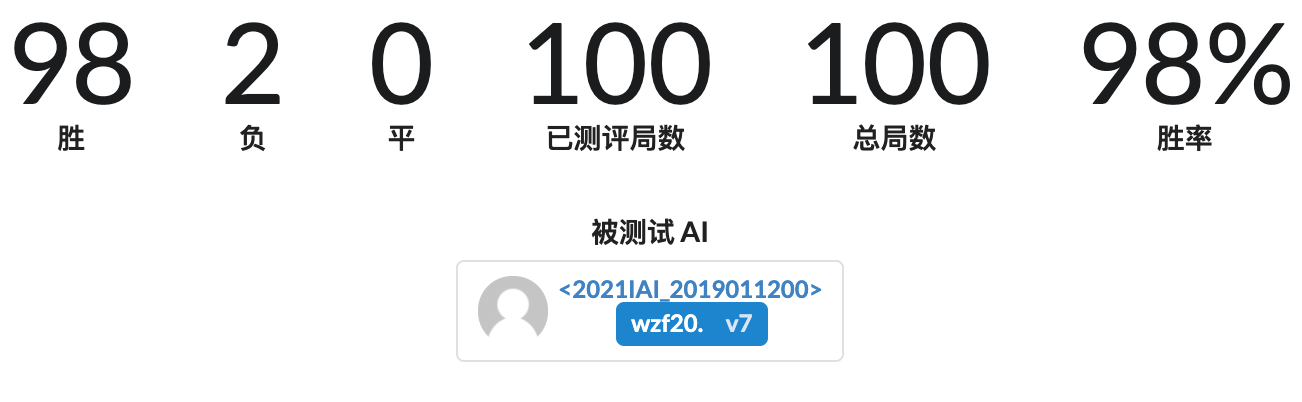
\includegraphics[width=1\textwidth]{1}
        \caption{全 AI 批量测试结果}
        \label{fig1}
    \end{figure}

    对应的批量测试序号为 $\pmb{\#10715}$,其中与 $94, 98$ 对战时后手负,其余均为胜利(先手全胜)。

    上述所有对抗中均未出现平局的情况。

    \section{总结}

    通过本次实验,我亲手实践了 UCT 信心上限树的算法。在实现过程中,我多次体会到了算法细节对于算法整体表现(胜率)的影响,特别是如双方胜负的判定、$Policy()$ 的计算等等。

    我也尝试进行了一些优化,从中特别体会到了人工智能搜索算法中,优化剪枝与搜索效率(耗时)之间的矛盾性,我们需要在其中尽量做到更好的平衡以得到尽量好的效果。

    最终,我实现的 AI 与样例 AI 的对抗结果,可以说较为令人满意,基本达到了预期效果。

    当然,最终版的模型在与许多高水平 AI 的对抗中仍有可改进的空间,这也是我的模型可以继续优化探究的部分。

    感谢老师和助教的悉心指导!
\end{document}
